\section{投影相机模型}\label{sec:投影相机模型}

三维计算机图形学中的一个基本问题是{\itshape 3D视见问题}:
如何将三维场景投影到二维图像上进行显示。
大多数经典方法都可以用$4\times4$的\keyindex{投影变换}{projective transformation}{transformation变换}矩阵来表达。
因此,我们将引入一个投影矩阵相机类\refvar{ProjectiveCamera}{},
然后在此基础上定义两个相机模型。
第一个实现了\keyindex{正交投影}{orthographic projection}{projection投影},
另一个实现了\keyindex{透视投影}{perspective projection}{projection投影}——
两种经典且广泛使用的\keyindex{投影}{projection}{}。
\begin{lstlisting}
`\initcode{Camera Declarations}{+=}\lastcode{CameraDeclarations}`
class `\initvar{ProjectiveCamera}{}` : public `\refvar{Camera}{}` {
public:
    `\refcode{ProjectiveCamera Public Methods}{}`
protected:
    `\refcode{ProjectiveCamera Protected Data}{}`
};
\end{lstlisting}

还有三个坐标系(总结于\reffig{6.1}中)对定义和讨论投影相机很有用。
\begin{itemize}
    \item \keyindex{屏幕空间}{screen space}{}:
          屏幕空间定义在胶片平面上。相机将相机空间中的物体投影到胶片平面上;
          \keyindex{屏幕窗口}{screen window}{}内的部分在生成的图像中是可见的。
          屏幕空间的深度$z$值从0变到1,分别对应近处和远处截平面的点。
          注意,虽然这称为“屏幕”空间,但它仍然是一个三维坐标系,因为$z$值是有意义的。
    \item \keyindex{规范化设备坐标}{normalized device coordinate}{}(NDC){\sffamily 空间}:
          这是被渲染的实际图像的坐标系。对于$x$和$y$,该空间范围从$(0,0)$变到$(1,1)$,
          其中$(0,0)$是图像的左上角。深度值与屏幕空间中的相同,线性变换将屏幕空间转换为NDC空间。
    \item \keyindex{栅格空间}{raster space}{}\sidenote{译者注:也称光栅空间。}:
          这与NDC空间几乎相同,除了$x$和$y$坐标从$(0,0)$变到(resolution.x, resolution.y)
          \sidenote{译者注:resolution指分辨率。}。
\end{itemize}

投影相机用$4\times4$矩阵在所有这些空间之间进行转换,
但具有特殊成像特性的相机不必用矩阵表示所有这些转换。
\begin{figure}[htbp]
    \centering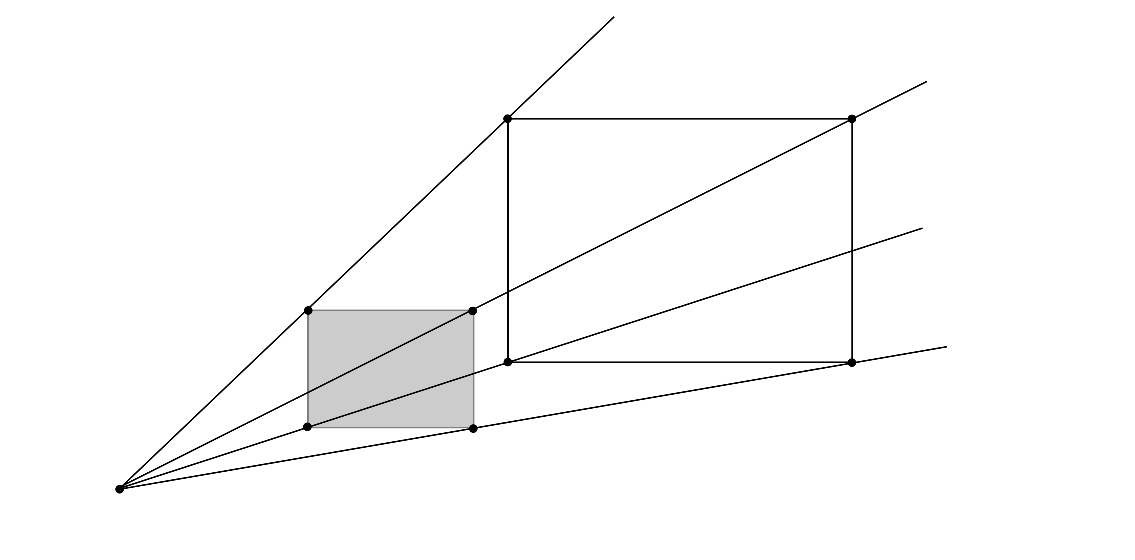
\includegraphics[width=0.75\linewidth]{chap06/Cameracoordinatespaces.eps}
    \put(-280,0){\small 相机空间:$(0,0,0)$}
    \put(-270,60){\small NDC:$(0,0,0)$}
    \put(-220,110){\small NDC:$(0,0,1)$}
    \put(-160,20){\small $z=\text{near}$}
    \put(-160,10){\small NDC:$(1,1,0)$}
    \put(-160,0){\small 栅格:$(\text{res}.x,\text{res}.y,0)$}
    \put(-70,35){\small $z=\text{far}$}
    \put(-70,25){\small NDC:$(1,1,1)$}
    \put(-70,15){\small 栅格:$(\text{res}.x,\text{res}.y,1)$}
    \caption{几个与相机相关的坐标空间常用于简化\protect\refvar{Camera}{}的实现。
        相机类持有它们之间的变换。世界空间中的场景物体由相机查看,它位于相机空间原点,并指向$+z$轴。
        近处和远处平面之间的物体被投影到相机空间中的胶片平面$z=\text{near}$上。
        胶片平面在栅格空间中$z=0$处,其中$x$和$y$范围从$(0,0)$变到(resolution.x, resolution.y)。
        规范化设备坐标(NDC)空间将栅格空间归一化,因此$x$和$y$范围从$(0,0)$变到$(1,1)$。}
    \label{fig:6.1}
\end{figure}

除了基类\refvar{Camera}{}要求的参数外,\refvar{ProjectiveCamera}{}还接收投影变换矩阵、
图像的屏幕空间范围以及与景深有关的额外参数。
\keyindex{景深}{depth of field}{}将在本节末尾介绍和实现,
它模拟了真实透镜系统中出现的失焦物体的模糊性。
\begin{lstlisting}
`\initcode{ProjectiveCamera Public Methods}{=}`
`\refvar{ProjectiveCamera}{}`(const `\refvar{AnimatedTransform}{}` &CameraToWorld, 
        const `\refvar{Transform}{}` &CameraToScreen, const `\refvar{Bounds2f}{}` &screenWindow,
        `\refvar{Float}{}` shutterOpen, `\refvar{Float}{}` shutterClose, `\refvar{Float}{}` lensr, `\refvar{Float}{}` focald,
        `\refvar{Film}{}` *film, const `\refvar{Medium}{}` *medium)
    : `\refvar{Camera}{}`(CameraToWorld, shutterOpen, shutterClose, film, medium),
      `\refvar{CameraToScreen}{}`(CameraToScreen) {
    `\refcode{Initialize depth of field parameters}{}`
    `\refcode{Compute projective camera transformations}{}`
}
\end{lstlisting}

\refvar{ProjectiveCamera}{}的实现将投影变换传递给这里展示的基类构造函数。
该变换给出了相机到屏幕的投影;
由此,构造函数能轻松算出从栅格空间到相机空间一路所需的其他变换。
\begin{lstlisting}
`\initcode{Compute projective camera transformations}{=}`
`\refcode{Compute projective camera screen transformations}{}`
`\refvar{RasterToCamera}{}` = `\refvar[Transform::Inverse]{Inverse}{}`(CameraToScreen) * `\refvar{RasterToScreen}{}`;
\end{lstlisting}
\begin{lstlisting}
`\initcode{ProjectiveCamera Protected Data}{=}\initnext{ProjectiveCameraProtectedData}`
`\refvar{Transform}{}` `\initvar{CameraToScreen}{}`, `\initvar{RasterToCamera}{}`;
\end{lstlisting}

在构造函数中唯一要计算的重要变换是屏幕到栅格的投影。
在下面的代码中,请注意变换的组成(从下往上看),
我们从屏幕空间的一个点开始,先平移使得屏幕左上角位于原点,
然后用屏幕宽度和高度的倒数进行缩放,
得到一个$x$和$y$坐标在0到1之间的点(这些是NDC坐标)。
最后,我们用栅格化分辨率进行缩放,这样我们最终就能完全覆盖
从$(0,0)$直到整个栅格分辨率的栅格范围。
这里一个重要细节是$y$坐标被该变换倒置了;
这是必要的,因为增加的$y$值在屏幕坐标中是向上移动但在栅格坐标中是向下的。
\begin{lstlisting}
`\initcode{Compute projective camera screen transformations}{=}`
`\refvar{ScreenToRaster}{}` = `\refvar{Scale}{}`(film->`\refvar{fullResolution}{}`.x, 
                       film->`\refvar{fullResolution}{}`.y, 1) *
    `\refvar{Scale}{}`(1 / (screenWindow.`\refvar{pMax}{}`.x - screenWindow.`\refvar{pMin}{}`.x),
          1 / (screenWindow.`\refvar{pMin}{}`.y - screenWindow.`\refvar{pMax}{}`.y), 1) *
    `\refvar{Translate}{}`(`\refvar{Vector3f}{}`(-screenWindow.`\refvar{pMin}{}`.x, -screenWindow.`\refvar{pMax}{}`.y, 0));
`\refvar{RasterToScreen}{}` = `\refvar[Transform::Inverse]{Inverse}{}`(`\refvar{ScreenToRaster}{}`);
\end{lstlisting}
\begin{lstlisting}
`\refcode{ProjectiveCamera Protected Data}{+=}\lastnext{ProjectiveCameraProtectedData}`
`\refvar{Transform}{}` `\initvar{ScreenToRaster}{}`, `\initvar{RasterToScreen}{}`;
\end{lstlisting}

\subsection{正交相机}\label{sub:正交相机}
\begin{lstlisting}
`\initcode{OrthographicCamera Declarations}{=}`
class `\initvar{OrthographicCamera}{}` : public `\refvar{ProjectiveCamera}{}` {
public:
    `\refcode{OrthographicCamera Public Methods}{}`
private:
    `\refcode{OrthographicCamera Private Data}{}`
};
\end{lstlisting}

定义在文件\href{https://github.com/mmp/pbrt-v3/blob/master/src/cameras/orthographic.h}{\ttfamily cameras/orthographic.h}和
\href{https://github.com/mmp/pbrt-v3/tree/master/src/cameras/orthographic.cpp}{\ttfamily cameras/orthographic.cpp}中的\keyindex{正交相机}{orthographic camera}{camera相机},
是基于正交投影变换的。
正交变换取场景中的一块矩形区域并将其投影到定义该区域之框的前方一面。
它不具有\keyindex{前缩}{foreshortening}{}效应——当物体远离时它们在成像平面上变小——
但它让平行线依然平行,并保留物体间的相对距离。
\reffig{6.2}{}展示了该立方体是如何定义场景可见区域的。
\begin{figure}[htbp]
    \centering%LaTeX with PSTricks extensions
%%Creator: Inkscape 1.1.1 (3bf5ae0d25, 2021-09-20)
%%Please note this file requires PSTricks extensions
\psset{xunit=.5pt,yunit=.5pt,runit=.5pt}
\begin{pspicture}(254.52000427,244.36999512)
{
\newrgbcolor{curcolor}{0 0 0}
\pscustom[linewidth=1,linecolor=curcolor]
{
\newpath
\moveto(5.5,162.19999512)
\lineto(5.5,8.15999512)
\lineto(160.1,8.15999512)
}
}
{
\newrgbcolor{curcolor}{0 0 0}
\pscustom[linestyle=none,fillstyle=solid,fillcolor=curcolor]
{
\newpath
\moveto(0,157.28999512)
\lineto(5.5,161.54999512)
\lineto(11.01,157.28999512)
\lineto(5.5,170.29999512)
\closepath
}
}
{
\newrgbcolor{curcolor}{0.65098041 0.65098041 0.65098041}
\pscustom[linestyle=none,fillstyle=solid,fillcolor=curcolor]
{
\newpath
\moveto(1.2,158.84999512)
\lineto(5.5,168.98999512)
\lineto(5.5,162.17999512)
\closepath
}
}
{
\newrgbcolor{curcolor}{0.40000001 0.40000001 0.40000001}
\pscustom[linestyle=none,fillstyle=solid,fillcolor=curcolor]
{
\newpath
\moveto(9.8,158.84999512)
\lineto(5.5,168.98999512)
\lineto(5.5,162.17999512)
\closepath
}
}
{
\newrgbcolor{curcolor}{0 0 0}
\pscustom[linestyle=none,fillstyle=solid,fillcolor=curcolor]
{
\newpath
\moveto(155.19,2.65999512)
\lineto(159.45,8.15999512)
\lineto(155.19,13.66999512)
\lineto(168.21,8.15999512)
\closepath
}
}
{
\newrgbcolor{curcolor}{0.65098041 0.65098041 0.65098041}
\pscustom[linestyle=none,fillstyle=solid,fillcolor=curcolor]
{
\newpath
\moveto(156.75,3.85999512)
\lineto(166.89,8.15999512)
\lineto(160.08,8.15999512)
\closepath
}
}
{
\newrgbcolor{curcolor}{0.40000001 0.40000001 0.40000001}
\pscustom[linestyle=none,fillstyle=solid,fillcolor=curcolor]
{
\newpath
\moveto(156.75,12.45999512)
\lineto(166.89,8.15999512)
\lineto(160.08,8.15999512)
\closepath
}
}
{
\newrgbcolor{curcolor}{0 0 0}
\pscustom[linewidth=1,linecolor=curcolor]
{
\newpath
\moveto(218.6000061,221.28999519)
\lineto(5.51999998,8.20999146)
}
}
{
\newrgbcolor{curcolor}{0 0 0}
\pscustom[linestyle=none,fillstyle=solid,fillcolor=curcolor]
{
\newpath
\moveto(211.24,221.70999512)
\lineto(218.14,220.82999512)
\lineto(219.02,213.92999512)
\lineto(224.33,227.01999512)
\closepath
}
}
{
\newrgbcolor{curcolor}{0.65098041 0.65098041 0.65098041}
\pscustom[linestyle=none,fillstyle=solid,fillcolor=curcolor]
{
\newpath
\moveto(213.19,221.95999512)
\lineto(223.4,226.08999512)
\lineto(218.59,221.27999512)
\closepath
}
}
{
\newrgbcolor{curcolor}{0.40000001 0.40000001 0.40000001}
\pscustom[linestyle=none,fillstyle=solid,fillcolor=curcolor]
{
\newpath
\moveto(219.27,215.87999512)
\lineto(223.4,226.08999512)
\lineto(218.59,221.27999512)
\closepath
}
}
{
\newrgbcolor{curcolor}{0.60000002 0.60000002 0.60000002}
\pscustom[linestyle=none,fillstyle=solid,fillcolor=curcolor]
{
\newpath
\moveto(62.79000092,116.37999725)
\lineto(172.98000336,116.37999725)
\lineto(172.98000336,50.18000031)
\lineto(62.79000092,50.18000031)
\closepath
}
}
{
\newrgbcolor{curcolor}{0 0 0}
\pscustom[linewidth=1,linecolor=curcolor]
{
\newpath
\moveto(62.79000092,116.37999725)
\lineto(172.98000336,116.37999725)
\lineto(172.98000336,50.18000031)
\lineto(62.79000092,50.18000031)
\closepath
}
}
{
\newrgbcolor{curcolor}{0 0 0}
\pscustom[linewidth=1,linecolor=curcolor,linestyle=dashed,dash=2]
{
\newpath
\moveto(254.02,131.03999512)
\lineto(143.83,131.03999512)
\lineto(143.83,197.23999512)
}
}
{
\newrgbcolor{curcolor}{0 0 0}
\pscustom[linewidth=1,linecolor=curcolor]
{
\newpath
\moveto(143.83,197.23999512)
\lineto(254.02,197.23999512)
\lineto(254.02,131.03999512)
}
}
{
\newrgbcolor{curcolor}{0 0 0}
\pscustom[linewidth=1,linecolor=curcolor]
{
\newpath
\moveto(62.79000092,116.37999725)
\lineto(143.83000183,197.23999405)
}
}
{
\newrgbcolor{curcolor}{0.60000002 0.60000002 0.60000002}
\pscustom[linestyle=none,fillstyle=solid,fillcolor=curcolor]
{
\newpath
\moveto(172.97999573,116.37999725)
\lineto(254.02000427,197.23999405)
}
}
{
\newrgbcolor{curcolor}{0 0 0}
\pscustom[linewidth=1,linecolor=curcolor]
{
\newpath
\moveto(172.97999573,116.37999725)
\lineto(254.02000427,197.23999405)
}
}
{
\newrgbcolor{curcolor}{0.60000002 0.60000002 0.60000002}
\pscustom[linestyle=none,fillstyle=solid,fillcolor=curcolor]
{
\newpath
\moveto(254.02000427,131.03999329)
\lineto(172.97999573,50.17999268)
}
}
{
\newrgbcolor{curcolor}{0 0 0}
\pscustom[linewidth=1,linecolor=curcolor]
{
\newpath
\moveto(254.02000427,131.03999329)
\lineto(172.97999573,50.17999268)
}
}
{
\newrgbcolor{curcolor}{0.60000002 0.60000002 0.60000002}
\pscustom[linestyle=none,fillstyle=solid,fillcolor=curcolor]
{
\newpath
\moveto(143.83000183,131.03999329)
\lineto(62.79000092,50.17999268)
}
}
{
\newrgbcolor{curcolor}{0 0 0}
\pscustom[linewidth=1,linecolor=curcolor,linestyle=dashed,dash=2]
{
\newpath
\moveto(143.83000183,131.03999329)
\lineto(62.79000092,50.17999268)
}
}
{
\newrgbcolor{curcolor}{0 0 0}
\pscustom[linestyle=none,fillstyle=solid,fillcolor=curcolor]
{
\newpath
\moveto(230.6197021,224.91641024)
\curveto(231.6822021,226.07266024)(232.2759521,226.57266024)(232.9947021,227.19766024)
\curveto(232.9947021,227.19766024)(234.2134521,228.26016024)(234.9322021,228.97891024)
\curveto(236.8384521,230.82266024)(237.2759521,231.79141024)(237.2759521,231.88516024)
\curveto(237.2759521,232.07266024)(237.0884521,232.07266024)(237.0572021,232.07266024)
\curveto(236.9009521,232.07266024)(236.8697021,232.04141024)(236.7447021,231.85391024)
\curveto(236.1509521,230.88516024)(235.7447021,230.57266024)(235.2759521,230.57266024)
\curveto(234.7759521,230.57266024)(234.5572021,230.88516024)(234.2447021,231.22891024)
\curveto(233.8697021,231.66641024)(233.5259521,232.07266024)(232.8697021,232.07266024)
\curveto(231.3697021,232.07266024)(230.4634521,230.22891024)(230.4634521,229.79141024)
\curveto(230.4634521,229.69766024)(230.5259521,229.57266024)(230.6822021,229.57266024)
\curveto(230.8697021,229.57266024)(230.9009521,229.66641024)(230.9634521,229.79141024)
\curveto(231.3384521,230.72891024)(232.4947021,230.72891024)(232.6509521,230.72891024)
\curveto(233.0572021,230.72891024)(233.4322021,230.60391024)(233.9009521,230.44766024)
\curveto(234.7134521,230.13516024)(234.9322021,230.13516024)(235.4322021,230.13516024)
\curveto(234.7134521,229.29141024)(233.0572021,227.85391024)(232.6822021,227.54141024)
\lineto(230.8697021,225.85391024)
\curveto(229.5259521,224.51016024)(228.8072021,223.38516024)(228.8072021,223.22891024)
\curveto(228.8072021,223.04141024)(229.0259521,223.04141024)(229.0572021,223.04141024)
\curveto(229.2134521,223.04141024)(229.2447021,223.07266024)(229.3697021,223.29141024)
\curveto(229.8384521,224.01016024)(230.4322021,224.54141024)(231.0884521,224.54141024)
\curveto(231.5259521,224.54141024)(231.7447021,224.35391024)(232.2447021,223.79141024)
\curveto(232.5572021,223.35391024)(232.9322021,223.04141024)(233.4947021,223.04141024)
\curveto(235.4947021,223.04141024)(236.6509521,225.57266024)(236.6509521,226.10391024)
\curveto(236.6509521,226.19766024)(236.5572021,226.32266024)(236.4009521,226.32266024)
\curveto(236.2134521,226.32266024)(236.1822021,226.19766024)(236.1197021,226.04141024)
\curveto(235.6509521,224.76016024)(234.3697021,224.38516024)(233.7134521,224.38516024)
\curveto(233.3384521,224.38516024)(232.9634521,224.51016024)(232.5572021,224.63516024)
\curveto(231.8697021,224.88516024)(231.5572021,224.97891024)(231.1509521,224.97891024)
\curveto(231.1197021,224.97891024)(230.8072021,224.97891024)(230.6197021,224.91641024)
\closepath
\moveto(230.6197021,224.91641024)
}
}
{
\newrgbcolor{curcolor}{0 0 0}
\pscustom[linestyle=none,fillstyle=solid,fillcolor=curcolor]
{
\newpath
\moveto(178.4398241,10.53037624)
\curveto(178.5648241,11.03037624)(179.0335741,12.87412624)(180.4085741,12.87412624)
\curveto(180.5023241,12.87412624)(181.0023241,12.87412624)(181.4085741,12.62412624)
\curveto(180.8460741,12.49912624)(180.4710741,12.03037624)(180.4710741,11.53037624)
\curveto(180.4710741,11.21787624)(180.6898241,10.84287624)(181.2210741,10.84287624)
\curveto(181.6585741,10.84287624)(182.2835741,11.18662624)(182.2835741,11.99912624)
\curveto(182.2835741,13.03037624)(181.1273241,13.31162624)(180.4398241,13.31162624)
\curveto(179.2835741,13.31162624)(178.5960741,12.24912624)(178.3460741,11.81162624)
\curveto(177.8460741,13.12412624)(176.7835741,13.31162624)(176.1898241,13.31162624)
\curveto(174.1273241,13.31162624)(172.9710741,10.74912624)(172.9710741,10.24912624)
\curveto(172.9710741,10.03037624)(173.1898241,10.03037624)(173.2210741,10.03037624)
\curveto(173.3773241,10.03037624)(173.4398241,10.09287624)(173.4710741,10.24912624)
\curveto(174.1585741,12.37412624)(175.4710741,12.87412624)(176.1585741,12.87412624)
\curveto(176.5335741,12.87412624)(177.2210741,12.68662624)(177.2210741,11.53037624)
\curveto(177.2210741,10.90537624)(176.8773241,9.59287624)(176.1585741,6.78037624)
\curveto(175.8460741,5.56162624)(175.1273241,4.71787624)(174.2523241,4.71787624)
\curveto(174.1273241,4.71787624)(173.6898241,4.71787624)(173.2523241,4.96787624)
\curveto(173.7523241,5.09287624)(174.1898241,5.49912624)(174.1898241,6.06162624)
\curveto(174.1898241,6.59287624)(173.7523241,6.74912624)(173.4710741,6.74912624)
\curveto(172.8460741,6.74912624)(172.3773241,6.24912624)(172.3773241,5.59287624)
\curveto(172.3773241,4.68662624)(173.3460741,4.28037624)(174.2210741,4.28037624)
\curveto(175.5648241,4.28037624)(176.2835741,5.68662624)(176.3148241,5.78037624)
\curveto(176.5648241,5.06162624)(177.2835741,4.28037624)(178.4710741,4.28037624)
\curveto(180.5335741,4.28037624)(181.6585741,6.84287624)(181.6585741,7.34287624)
\curveto(181.6585741,7.56162624)(181.5023241,7.56162624)(181.4398241,7.56162624)
\curveto(181.2523241,7.56162624)(181.2210741,7.46787624)(181.1585741,7.34287624)
\curveto(180.5023241,5.18662624)(179.1585741,4.71787624)(178.5335741,4.71787624)
\curveto(177.7523241,4.71787624)(177.4398241,5.34287624)(177.4398241,6.03037624)
\curveto(177.4398241,6.46787624)(177.5335741,6.90537624)(177.7523241,7.78037624)
\closepath
\moveto(178.4398241,10.53037624)
}
}
{
\newrgbcolor{curcolor}{0 0 0}
\pscustom[linestyle=none,fillstyle=solid,fillcolor=curcolor]
{
\newpath
\moveto(12.9314461,185.17229724)
\curveto(13.0251961,185.45354724)(13.0251961,185.48479724)(13.0251961,185.64104724)
\curveto(13.0251961,185.98479724)(12.7439461,186.17229724)(12.4314461,186.17229724)
\curveto(12.2439461,186.17229724)(11.9314461,186.04729724)(11.7439461,185.76604724)
\curveto(11.7126961,185.64104724)(11.5251961,185.04729724)(11.4626961,184.67229724)
\curveto(11.3064461,184.17229724)(11.1814461,183.60979724)(11.0564461,183.07854724)
\lineto(10.1501961,179.48479724)
\curveto(10.0876961,179.20354724)(9.2126961,177.79729724)(7.9001961,177.79729724)
\curveto(6.9001961,177.79729724)(6.6814461,178.67229724)(6.6814461,179.42229724)
\curveto(6.6814461,180.32854724)(7.0251961,181.57854724)(7.6814461,183.32854724)
\curveto(7.9939461,184.14104724)(8.0876961,184.35979724)(8.0876961,184.76604724)
\curveto(8.0876961,185.64104724)(7.4626961,186.39104724)(6.4626961,186.39104724)
\curveto(4.5564461,186.39104724)(3.8376961,183.48479724)(3.8376961,183.32854724)
\curveto(3.8376961,183.10979724)(4.0251961,183.10979724)(4.0564461,183.10979724)
\curveto(4.2751961,183.10979724)(4.2751961,183.17229724)(4.3689461,183.48479724)
\curveto(4.9314461,185.35979724)(5.7126961,185.95354724)(6.4001961,185.95354724)
\curveto(6.5564461,185.95354724)(6.9001961,185.95354724)(6.9001961,185.32854724)
\curveto(6.9001961,184.82854724)(6.6814461,184.29729724)(6.5564461,183.92229724)
\curveto(5.7439461,181.79729724)(5.4001961,180.67229724)(5.4001961,179.73479724)
\curveto(5.4001961,177.95354724)(6.6501961,177.35979724)(7.8376961,177.35979724)
\curveto(8.6189461,177.35979724)(9.2751961,177.70354724)(9.8376961,178.26604724)
\curveto(9.5876961,177.23479724)(9.3376961,176.23479724)(8.5564461,175.17229724)
\curveto(8.0251961,174.51604724)(7.2751961,173.92229724)(6.3689461,173.92229724)
\curveto(6.0876961,173.92229724)(5.1814461,173.98479724)(4.8376961,174.76604724)
\curveto(5.1501961,174.76604724)(5.4314461,174.76604724)(5.6814461,175.01604724)
\curveto(5.9001961,175.17229724)(6.0876961,175.45354724)(6.0876961,175.82854724)
\curveto(6.0876961,176.45354724)(5.5564461,176.51604724)(5.3689461,176.51604724)
\curveto(4.9001961,176.51604724)(4.2439461,176.20354724)(4.2439461,175.23479724)
\curveto(4.2439461,174.23479724)(5.1189461,173.48479724)(6.3689461,173.48479724)
\curveto(8.4001961,173.48479724)(10.4626961,175.29729724)(11.0251961,177.54729724)
\closepath
\moveto(12.9314461,185.17229724)
}
}
\end{pspicture}

    \caption{正交视见体是相机空间中的轴对齐框,
        其定义使该区域内的物体投影到该框$z=\text{near}$的一面上。}
    \label{fig:6.2}
\end{figure}

\reffig{6.3}比较了用正交投影和下节定义的透视投影来渲染的结果
\sidenote{译者注:原图为exr格式,此处转换为png格式以便制作插图,
    图像细节和色域可能发生细微变化。后续均作此处理,读者可到原书官网查看原图。}。
\begin{figure}[htbp]
    \centering
    \subfloat[正交]{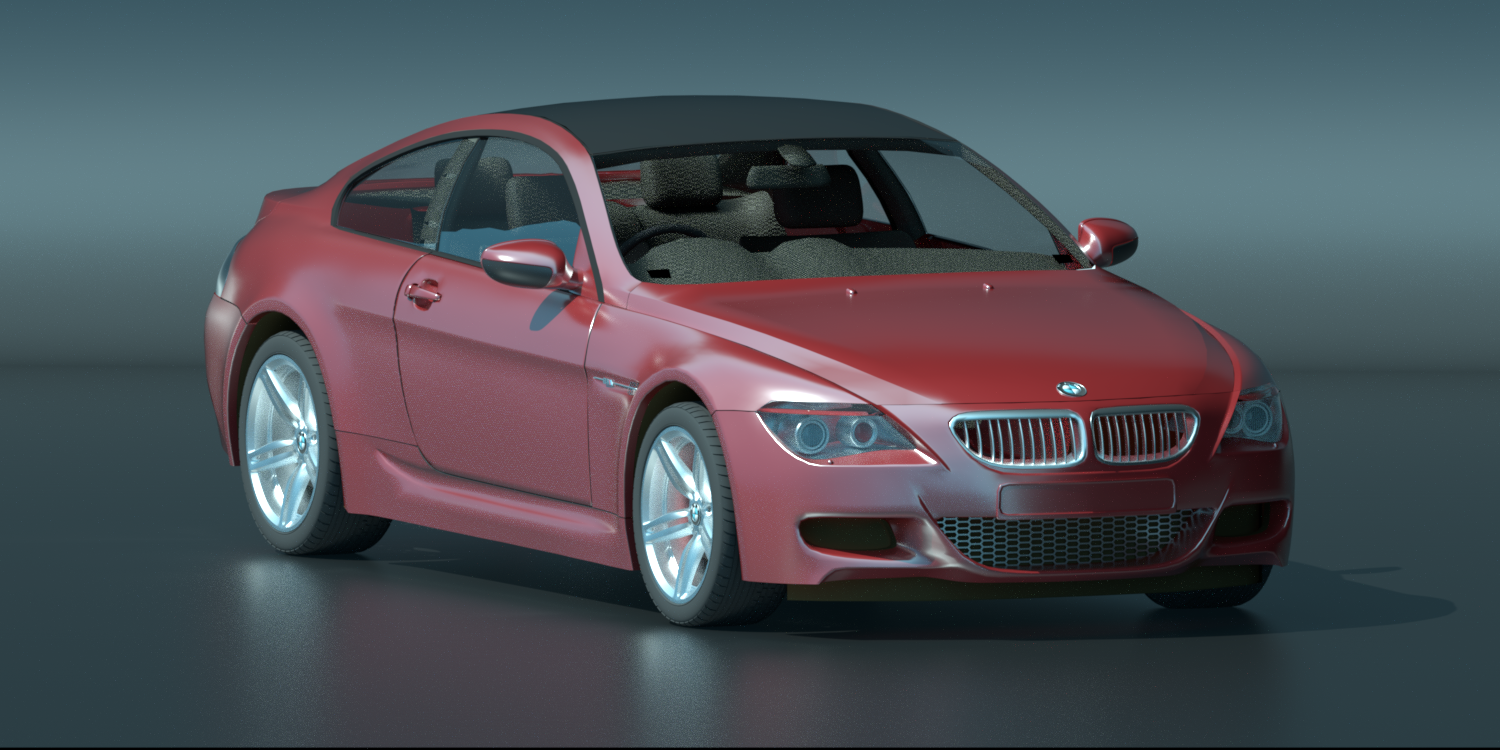
\includegraphics[width=\linewidth]{chap06/car-ortho.png}\label{fig:6.3.1}}\\
    \subfloat[透视]{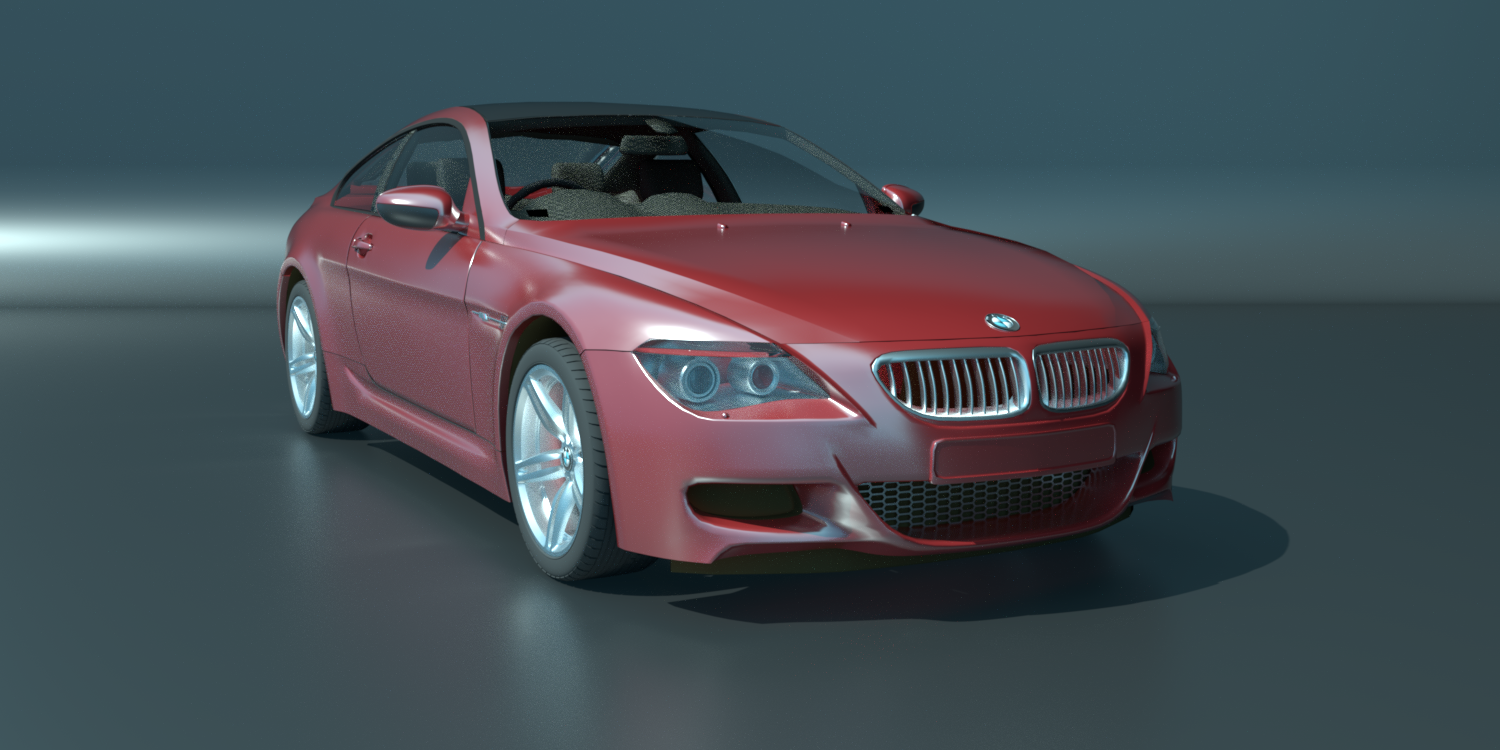
\includegraphics[width=\linewidth]{chap06/car-perspective.png}\label{fig:6.3.2}}
    \caption{用不同相机模型渲染的汽车模型。用(a)正交和(b)透视相机从同一视点渲染汽车。
        缺少前缩使得正交视角看起来深度更少,但它保留了平行线这一很有用的特性。}
    \label{fig:6.3}
\end{figure}

\subsection{薄透镜模型与景深}\label{sub:薄透镜模型与景深}
